\section{Sesión 2}
% SESSION II: FL ATTACKS
Para esta sesión, se ha utilizado de nuevo la configuracion de entrenamiento de DFL non-IID de la sesión anterior. Se han realizado con ella los siguientes experimentos:
\begin{itemize}
    \item Ataque de \textit{model poisoning} con 10\% de ruido gaussiano.
    \item Ataque de \textit{label flipping} con 80\% de muestras envenenadas.
\end{itemize}
Para cada uno de los ataques, compararemos con un 20\% y un 50\% de clientes maliciosos. 


\subsection{Model poisoning}

En este ataque, los clientes maliciosos añaden ruido gaussiano a sus modelos locales antes de enviarlos para la agregación. Este ruido degrada la calidad de las actualizaciones, afectando al proceso de convergencia.
\vspace{1mm}

Los resultados obtenidos se muestran en la Figura \ref{fig:model_poisoning}:

\vspace{1mm}
\noindent
\begin{minipage}{\textwidth}
    \centering
    \begin{tabular}{cc}
        \textbf{20\% nodos maliciosos} & \textbf{50\% nodos maliciosos} \\
        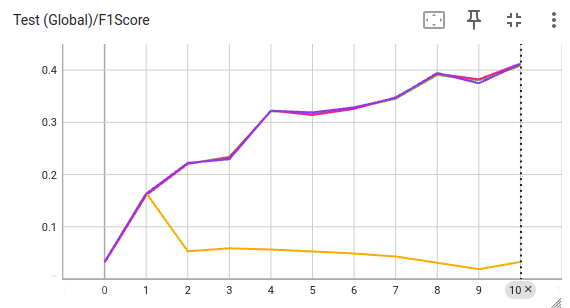
\includegraphics[width=0.4\textwidth]{images/model_poisoning_20.png} &
        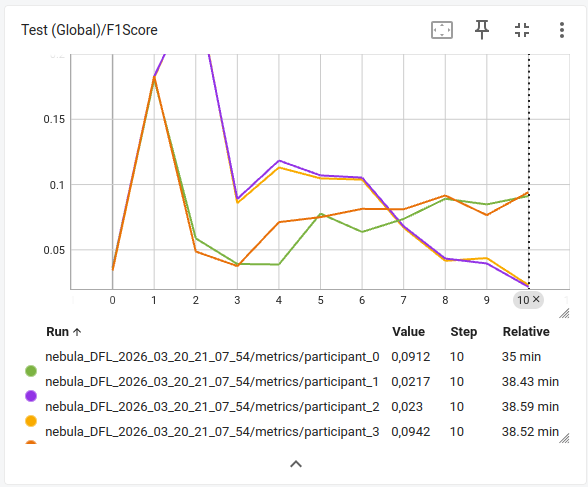
\includegraphics[width=0.4\textwidth]{images/model_poisoning_50.png} \\
    \end{tabular}
    \captionof{figure}{Impacto del ataque de \textit{model poisoning} con diferentes porcentajes de nodos maliciosos.}
    \label{fig:model_poisoning}
\end{minipage}
\vspace{1mm}

Se observa que el impacto del ataque aumenta significativamente con el número de nodos maliciosos, provocando una notable inestabilidad:

\begin{itemize}
    \item Con un 20\% de nodos maliciosos, la mayoría de los participantes logra converger hacia un F1-score aproximado de 0.41. Sin embargo, el nodo atacante queda rezagado con un valor de apenas 0.03 porque realiza el test después de introducir el ruido al modelo recibido por el agregador.
    \item Con un 50\% de nodos maliciosos, la convergencia se ve gravemente afectada. La gráfica muestra fuertes oscilaciones y una degradación final, desplomando el F1-score a valores casi nulos de entre 0.02 y 0.09 en el último paso.
\end{itemize}

%Las matrices de confusión reflejan un aumento en los errores de clasificación generalizados, sin afectar a clases específicas de forma predominante, lo cual es consistente con la naturaleza no dirigida del ruido gaussiano.

\subsection{Label flipping}

En este caso, los nodos maliciosos alteran las etiquetas de un 80\% de sus muestras de entrenamiento de manera aleatoria. Este ataque introduce información incorrecta directamente en el proceso de aprendizaje.
\vspace{1mm}

Los resultados se muestran en la Figura \ref{fig:label_flipping}:

\vspace{1mm}
\noindent
\begin{minipage}{\textwidth}
    \centering
    \begin{tabular}{cc}
        \textbf{20\% nodos maliciosos} & \textbf{50\% nodos maliciosos} \\
        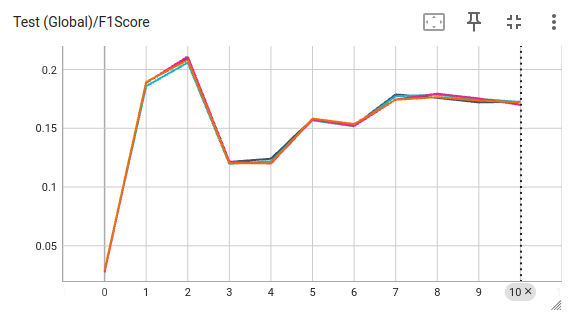
\includegraphics[width=0.4\textwidth]{images/label_flipping_20.png} &
        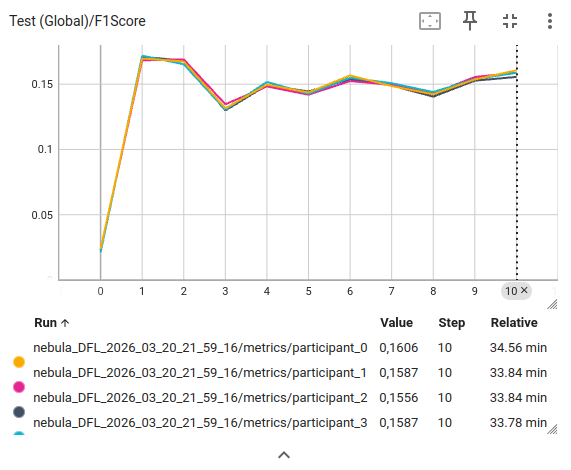
\includegraphics[width=0.4\textwidth]{images/label_flipping_50.png} \\
    \end{tabular}
    \captionof{figure}{Impacto del ataque de \textit{label flipping} con diferentes porcentajes de nodos maliciosos.}
    \label{fig:label_flipping}
\end{minipage}
\vspace{1mm}

En este escenario, el impacto reduce el rendimiento pero mantiene un entrenamiento más estable:

\begin{itemize}
    \item Con un 20\% de nodos maliciosos, el modelo presenta una convergencia estable agrupada para todos los clientes, alcanzando un F1-score final en torno a 0.48.
    \item Con un 50\% de nodos maliciosos, el modelo logra converger pero el rendimiento se desploma, estancándose de manera uniforme en un F1-score de 0.15.
\end{itemize}

%Las matrices de confusión muestran patrones de error más estructurados, con confusión sistemática entre clases, lo que indica que el modelo aprende relaciones incorrectas debido a las etiquetas alteradas.

\subsection{Comparación y análisis}

Comparando ambos ataques y configuraciones con los datos obtenidos, se extraen las siguientes conclusiones:

\begin{itemize}
    \item Contrario a lo que se podría intuir en un inicio, el ataque de \textit{model poisoning} genera un escenario más desestabilizador y destructivo en altas proporciones (50\%) que el de \textit{label flipping}. Mientras el primero destruye la convergencia (F1-score $\leq 0,09$), el segundo logra engañar al modelo llevándolo a una convergencia falsa pero ligeramente superior (F1-score $\sim 0,16$).
    \item A medida que aumenta el porcentaje de clientes maliciosos (20\% $\rightarrow$ 50\%), la métrica final cae drásticamente en ambos ataques: de $\sim$0,41 a $\leq$0,09 en \textit{model poisoning}, y de $\sim$0,48 a $\sim$0,16 en \textit{label flipping}.
    %\item En comparación con los resultados de la sesión 1, donde el caso non-IID ya presentaba dificultades de convergencia, los ataques agravan aún más este problema y resaltan la fragilidad de estas redes frente a actores bizantinos.
    \item En la sesión anterior, el entorno DFL ideal (IID) alcanzaba un F1-score de $\sim$0,67, mientras que la simple introducción de heterogeneidad en los datos (DFL non-IID base) lo reducía a $\sim$0,50. Al introducir condiciones de ataque sobre este último escenario, la degradación se amplifica: en la condición de ataque más leve (20\% \textit{label flipping}), el F1-score ya cae por debajo del caso base a $\sim$0,48. En las condiciones de ataque más severas (50\% \textit{model poisoning}), el modelo se desploma hasta un 0,02. Esto evidencia que los entornos non-IID son frágiles ante actualizaciones maliciosas, ya que a la agregación le resulta mucho más difícil distinguir entre una variación legítima (datos sesgados) y un ataque intencionado.

\end{itemize}

% En cuanto a la evolución temporal:

% \begin{itemize}
%     \item En escenarios de \textit{model poisoning} se evidencia un claro comportamiento errático (oscilaciones abruptas en el caso del 50\%) y particiones en el aprendizaje global (como el nodo rezagado en el caso del 20\%).
%     \item El \textit{label flipping}, por el contrario, fomenta una ilusión de estabilidad, ya que todos los participantes convergen de manera solidaria pero hacia un modelo que ha interiorizado lógicas de clasificación erróneas.
% \end{itemize}

% En resumen, los ataques afectan tanto a la calidad final del modelo como a la dinámica de entrenamiento, siendo el entorno non-IID especialmente vulnerable debido a la ya existente heterogeneidad de los datos.

Matriz de atacante